\section{2-Choices}
\label{2Choices}

As we have already written in this transition rule, The selected agent u observes the opinions of two other agents selected uniformly at random. If their opinions coincide, agent u adopts it. Otherwise it retains its original opinion.
We have done four types of plot, that are going to be shown also for the other transition rules:
\begin{itemize}
     \item The first one is a line plot based on the time that the simulation has taken in order to arrive at that status. So in the x-axis there is the time;
     \item The second one is always a line plot based on the number of iterations done by the simulation in order to arrive at that status. For the 2-choices iteration rule we have decided to fetch the data each 200 000 iterations;
     \item The third one is a bar plot based on the number of iterations;
     \item The last one is a bar plot based on the time spent by the algorithm to do the simulations.
\end{itemize}

% \begin{center}
%      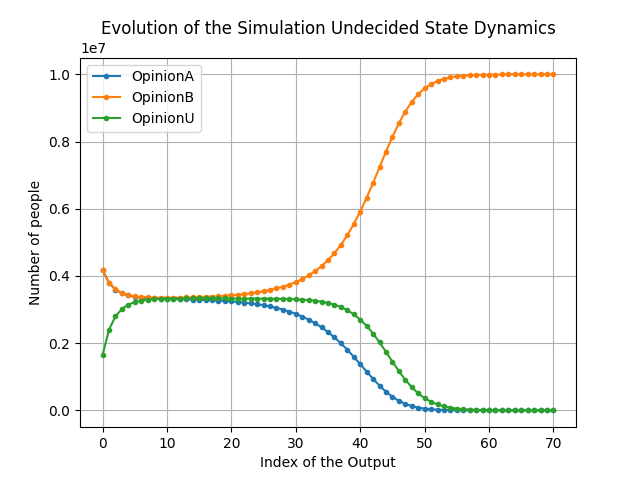
\includegraphics[width=0.87\textwidth,height=0.40\textheight]{img/svg/Undecided/100mln/withoutTime.png}
%     \blfootnote{Immagine \href{https://github.com/Life-planner/Documentazione/blob/main/D3/img/png/DCL/Abbonamento.png}{PNG}/\href{https://github.com/Life-planner/Documentazione/blob/main/D3/img/svg/DCL/Abbonamento.svg}{SVG} Diagramma delle classi "Abbonamento"}
% \end{center}

% \begin{figure}[H]
%      \centering
%      \href{https://www.figma.com/proto/cO66hx25OizBABGtWp8XlT/Planify?node-id=160%3A290&scaling=scale-down&page-id=0%3A1&starting-point-node-id=25%3A82}{\includegraphics[width=0.9\textwidth]{img/FrontEnd/Eventi/SottoAttivita.png}}
%      \caption{Figura 5: schermata quando si apre la sezione "Eventi"}
%  \end{figure}
%  \blfootnote{Immagine \href{https://github.com/Life-planner/Documentazione/blob/main/D1/img/FrontEnd/Eventi/SottoAttivita.png}{PNG} schermata eventi}
%  \blfootnote{Immagine \href{https://github.com/Life-planner/Documentazione/blob/main/D1/img/FrontEnd/Eventi/Calendario/CreaCalendario.png}{PNG} schermata calendari}
%  \begin{figure}[H]
%      \centering
%      \href{https://www.figma.com/proto/cO66hx25OizBABGtWp8XlT/Planify?node-id=160%3A290&scaling=scale-down&page-id=0%3A1&starting-point-node-id=25%3A82}{\includegraphics[width=0.9\textwidth]{img/FrontEnd/Eventi/Calendario/CreaCalendario.png}}
%      \caption{Figura 5: schermata quando si seleziona uno dei comandi o un'attività della lista}
%  \end{figure}

\begin{figure}[H]
     \centering
     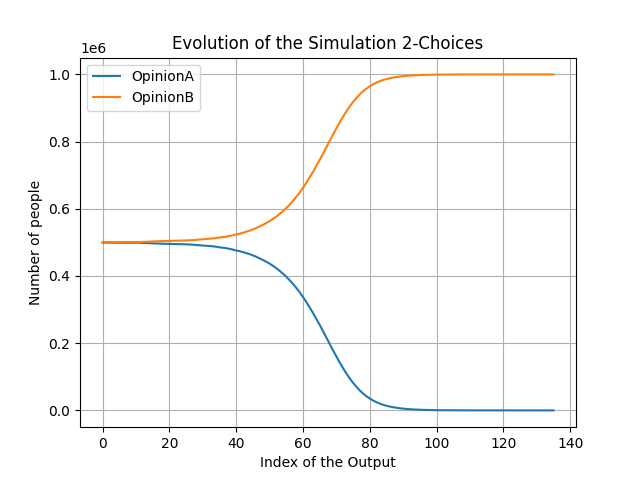
\includegraphics[width=0.78\textwidth,height=0.32\textheight]{img/svg/2Choices/1mln/withoutTime.png}
     \caption{Simulation done with 1mln agents, output each 200 000 iteration}
\end{figure}
%  \blfootnote{Immagine \href{https://github.com/Life-planner/Documentazione/blob/main/D1/img/FrontEnd/Eventi/SottoAttivita.png}{PNG} schermata eventi}
%  \blfootnote{Immagine \href{https://github.com/Life-planner/Documentazione/blob/main/D1/img/FrontEnd/Eventi/Calendario/CreaCalendario.png}{PNG} schermata calendari}
\begin{figure}[H]
     \centering
     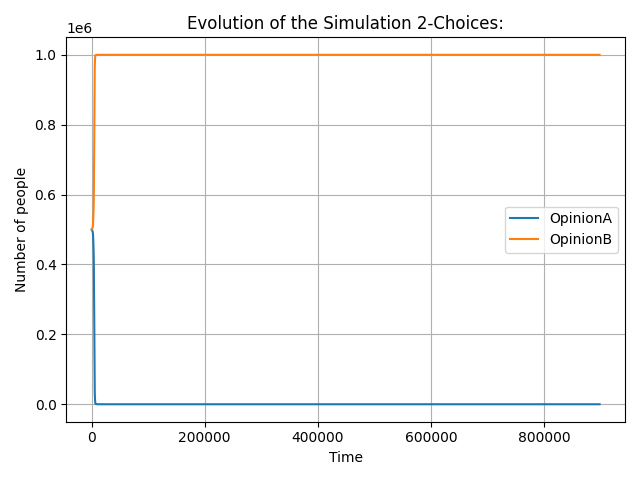
\includegraphics[width=0.75\textwidth,height=0.32\textheight]{img/svg/2Choices/1mln/withTime.png}
     \caption{Simulation done with 1mln of agents, Time calculated in ms}
\end{figure}

% \begin{figure}[!ht]
%      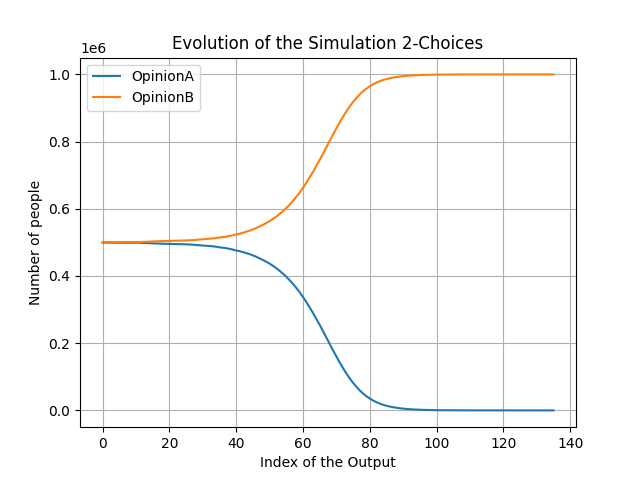
\includegraphics[width=0.48\textwidth,height=0.35\textheight]{img/svg/2Choices/1mln/withoutTime.png}
%      \centering
%      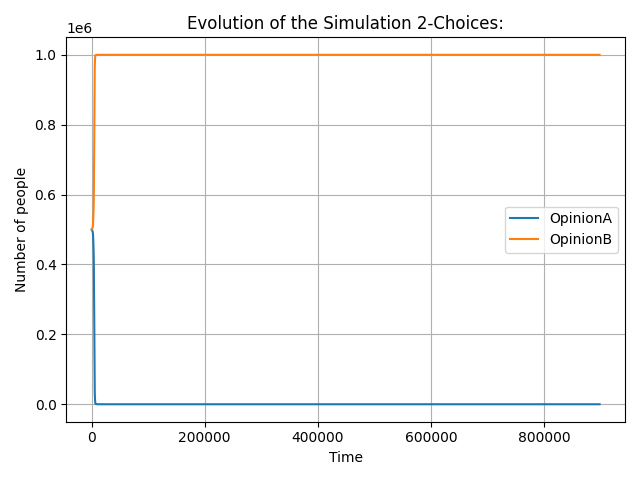
\includegraphics[width=0.48\textwidth,height=0.35\textheight]{img/svg/2Choices/1mln/withTime.png}
% \end{figure}

As we can see from the plots, in the first plot the evolution faster, this happens because the time increases faster compared to the number of iterations (or index of the output) and for this reason also the y values increase faster in the first plot!
Anyway, from the plot with the time, we can notice that the algorithm takes only a few seconds in order to finish the procedure.

\begin{figure}[H]
     \centering
     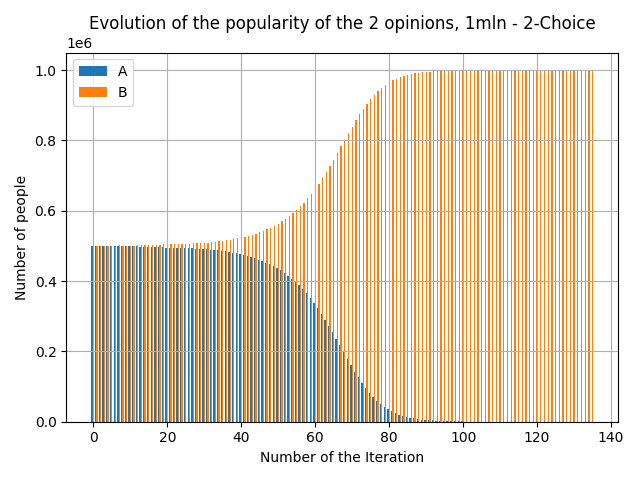
\includegraphics[width=0.80\textwidth,height=0.37\textheight]{img/svg/2Choices/1mln/barChart.png}
     \caption{Simulation done with 1mln of agents}
\end{figure}

From the bar plot we can immediately notice one thing. At the beginning, the growth of one opinion compared to the other is slower. If we think about it a bit, we can conclude that it is something really normal. In fact, for each iteration the algorithm takes three agents. The first agent is going to change his opinion if and only if the other agents have the same opinion.
At the start of this algorithm, we decided to put the same probability (0.5) for the choice of the starting opinion of an agent. For this reason, at the beginning of the simulation the number of agents with opinion “A” and agent with opinion “B” is approximately the same.
As a result, in the first iterations there is a high probability that the two agents have different opinions and for this reason the first agent doesn’t change his opinion and the number of “A” and “B” doesn’t change.\\
On the other hand the plots below show the behavior of the algorithm with 10mln and 100mln of agents. As we can see the evolution of the line is approximately the same as with 1mln agents, for this reason there isn’t much to say about them.

\begin{figure}[!ht]
     \includegraphics[width=0.40\textwidth,height=0.17\textheight]{img/svg/2Choices/10mln/withoutTime.png}
     \centering
     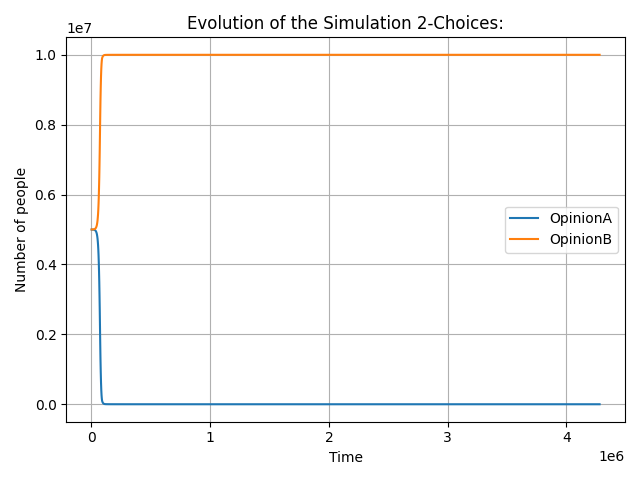
\includegraphics[width=0.40\textwidth,height=0.17\textheight]{img/svg/2Choices/10mln/withtTime.png}
     \caption{Simulation done with 10mln agents, Time in ms}
\end{figure}
\newpage
\begin{figure}[!ht]
     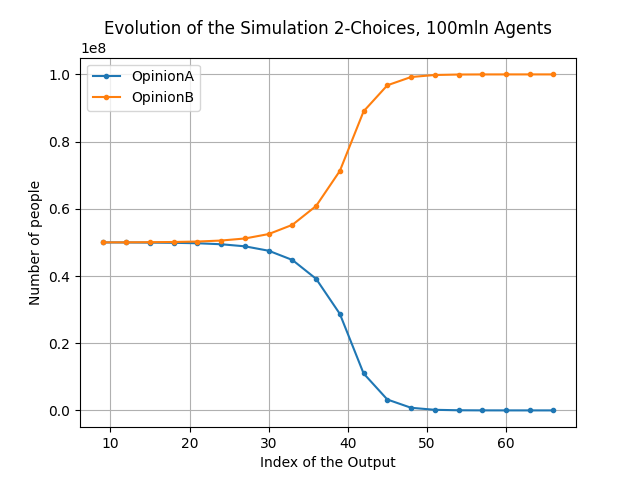
\includegraphics[width=0.40\textwidth,height=0.17\textheight]{img/svg/2Choices/100mln/withoutTime.png}
     \centering
     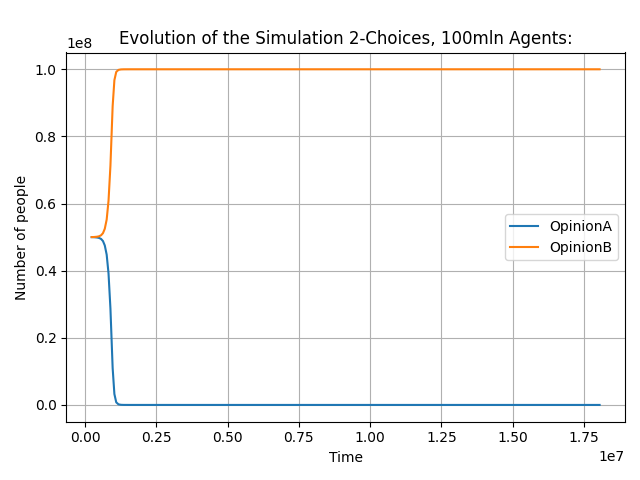
\includegraphics[width=0.40\textwidth,height=0.17\textheight]{img/svg/2Choices/100mln/withTime.png}
     \caption{Simulation done with 100mln agents, Time in ms}
\end{figure}
On the contrary, the following bar plot is really interesting because it shows the difference in the time taken by the algorithm to do the transition rule 2-Choice. We can see that the time, for example from 1mln to 10mln, changes for a factor of a little more than 1/4, that anyway is less than the factor 1/10 that there is between the number of agents in the 2 simulations. This means that it’s true that time and dimension of the input are directly proportional, but not of the same factor!

\begin{figure}[H]
     \centering
     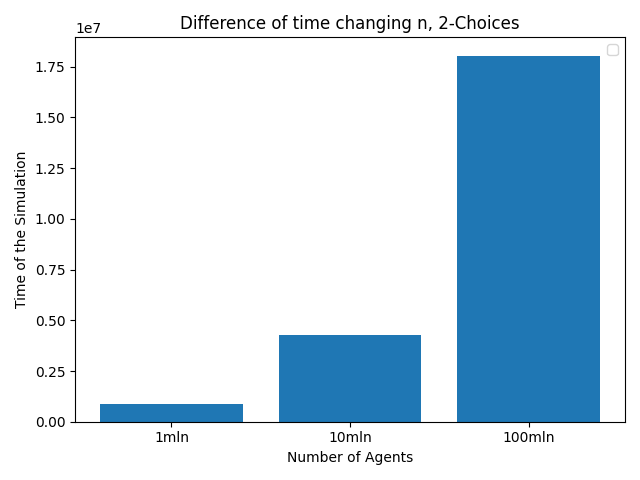
\includegraphics[width=0.80\textwidth,height=0.37\textheight]{img/svg/2Choices/TimeDifferenceN.png}
\end{figure}

\subsection[0.5-0.75 2Choices]{Comparison between 0.5 and 0.75, 2-Choices simulation}
In order to determine the effects of the starting ratio, we also did some tests with 0.75 starting probability, so for each agent there is a probability of 75\% to choose A and 25\% to choose "B" at the start of the simulation. After the tests, we observed that both the number of iterations and time decreased for 0.75 probability, as we could expected. The consensus happened in around 300,000,000 iterations when the starting probability was 0.5. For the 0.75, this number decreased to around 135,000,000. Similarly, while the old timing was 4 million ms, after setting the starting ratio to 0.75, it decreased to around 2 million ms.
\newpage
\begin{figure}[H]
     \centering
     \includegraphics[width=0.60\textwidth,height=0.23\textheight]{img/svg/0.75/2Choices/withoutTime.png}
     \caption{Probability A 0.75, output each 5 million iterations}
\end{figure}
\begin{figure}[H]
     \centering
     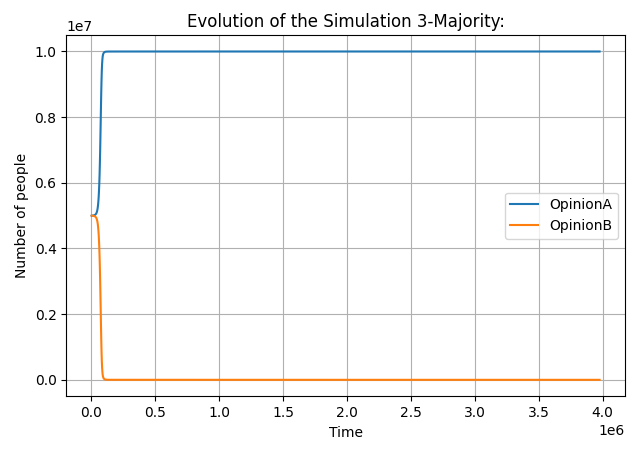
\includegraphics[width=0.60\textwidth,height=0.23\textheight]{img/svg/0.75/2Choices/withTime.png}
     \caption{Probability A 0.75, Time calculated in ms}
\end{figure}
\begin{figure}[H]
     \centering
     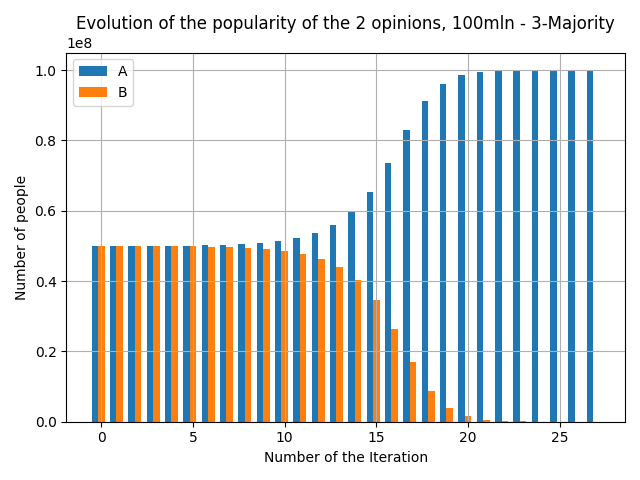
\includegraphics[width=0.60\textwidth,height=0.23\textheight]{img/svg/0.75/2Choices/barChart.png}
     \caption{Probability A 0.75, Done with 10mln of agents}
\end{figure}

% \begin{figure}[H]
%      \centering
%      \includegraphics[width=0.57\textwidth,height=0.22\textheight]{img/svg/2Choices/10mln/withoutTime.png}
%      \caption{Simulation done with 1mln Agents}
% \end{figure}
% \begin{figure}[H]
%      \centering
%      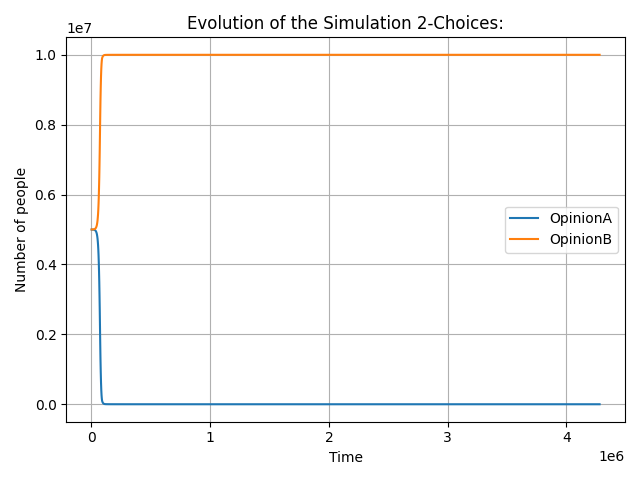
\includegraphics[width=0.75\textwidth,height=0.32\textheight]{img/svg/2Choices/10mln/withtTime.png}
%      \caption{Simulation done with 10mln of Agents, Time calculated in ms}
% \end{figure}